\hypertarget{temperature__sensor___terciopelo_8pde}{
\section{/Users/nikki/nublabs/nub.datalogger/hardware/temperature\_\-sensor\_\-Terciopelo/temperature\_\-sensor\_\-Terciopelo.pde File Reference}
\label{temperature__sensor___terciopelo_8pde}\index{/Users/nikki/nublabs/nub.datalogger/hardware/temperature\_\-sensor\_\-Terciopelo/temperature\_\-sensor\_\-Terciopelo.pde@{/Users/nikki/nublabs/nub.datalogger/hardware/temperature\_\-sensor\_\-Terciopelo/temperature\_\-sensor\_\-Terciopelo.pde}}
}
{\tt \#include \char`\"{}name.h\char`\"{}}\par
{\tt \#include \char`\"{}globals.h\char`\"{}}\par
{\tt \#include \char`\"{}communications\_\-definitions.h\char`\"{}}\par
{\tt \#include $<$stdio.h$>$}\par


Include dependency graph for temperature\_\-sensor\_\-Terciopelo.pde:\nopagebreak
\begin{figure}[H]
\begin{center}
\leavevmode
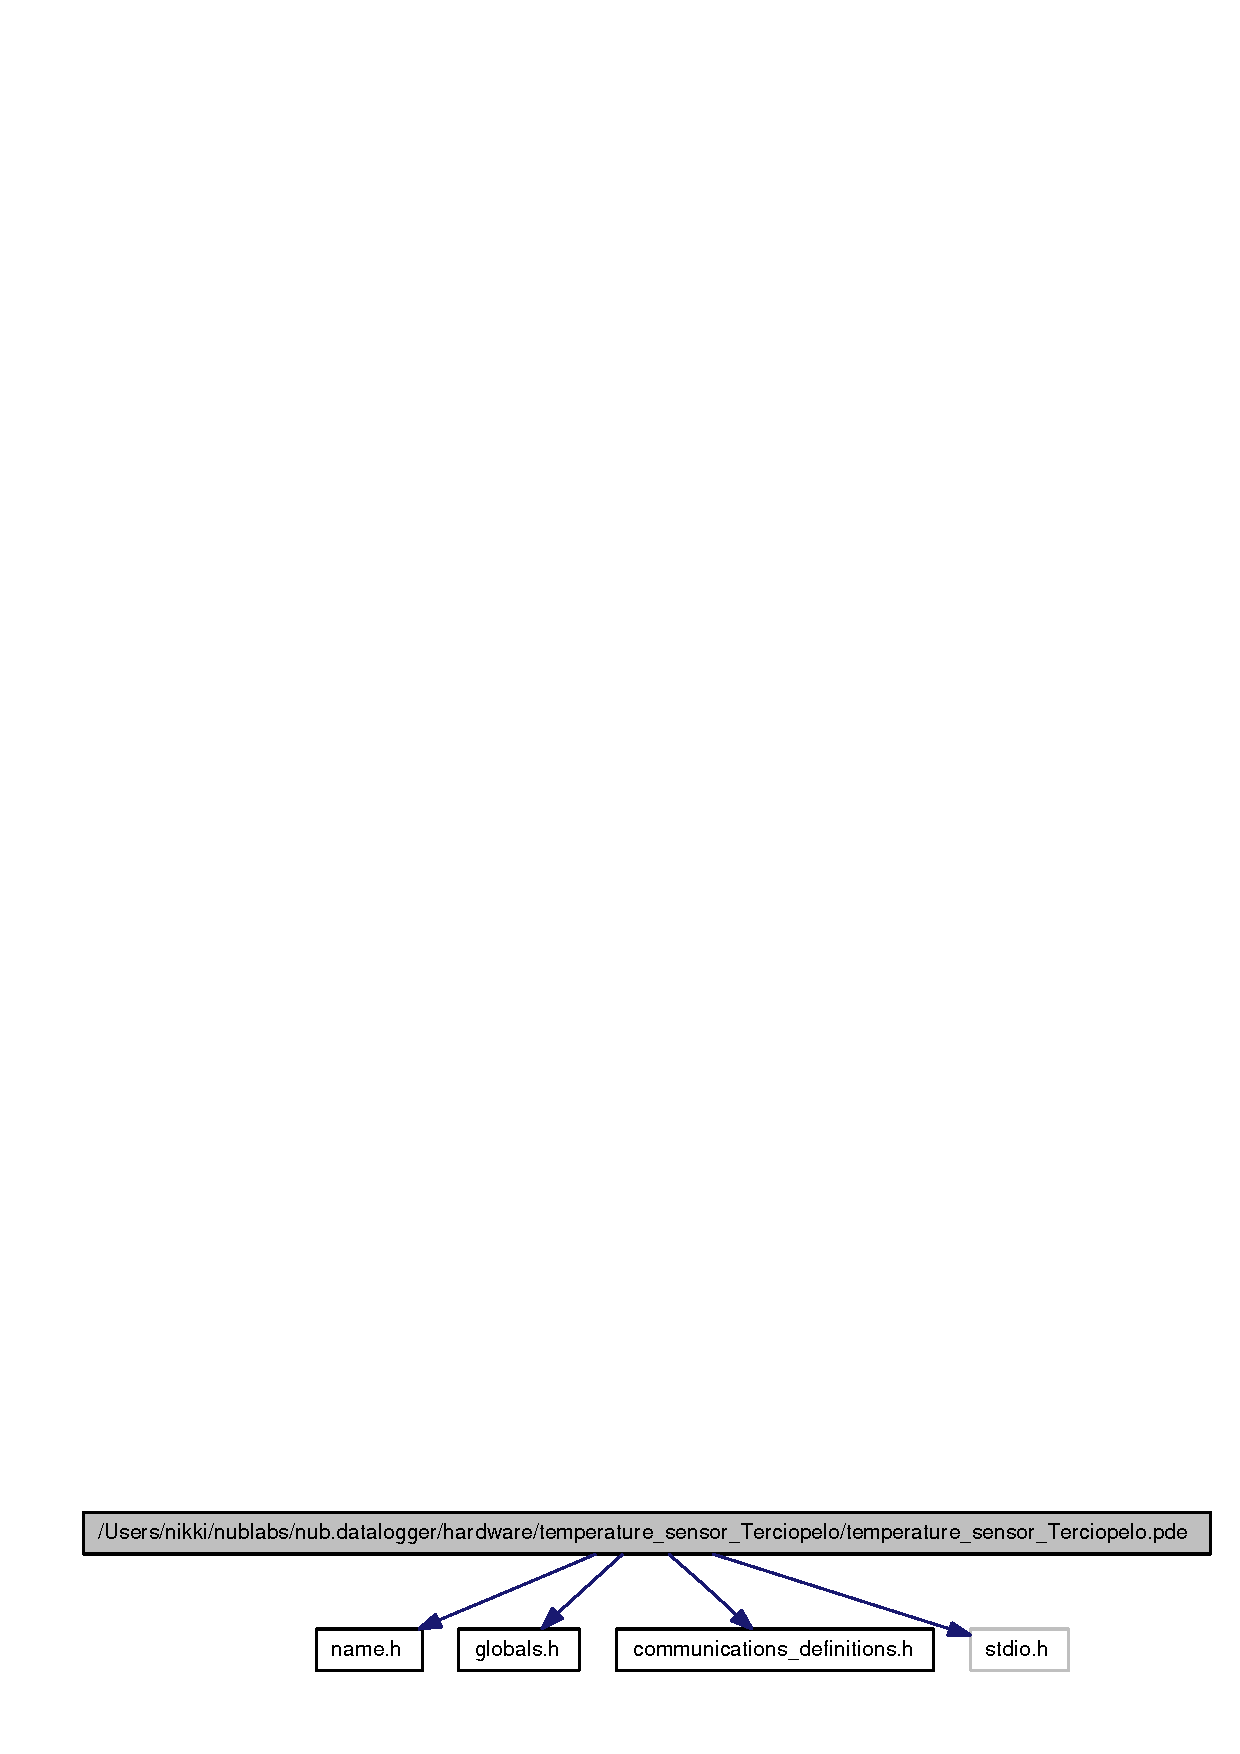
\includegraphics[width=292pt]{temperature__sensor___terciopelo_8pde__incl}
\end{center}
\end{figure}
\subsection*{Defines}
\begin{CompactItemize}
\item 
\#define \hyperlink{temperature__sensor___terciopelo_8pde_658c2878485cfe5cc625d283a6d34bc1}{XBEE\_\-SLEEP}~2
\item 
\#define \hyperlink{temperature__sensor___terciopelo_8pde_b2de299215608c2a35f0feb86adc2f6f}{SAMPLE\_\-BUTTON}~3
\item 
\#define \hyperlink{temperature__sensor___terciopelo_8pde_eb7a7ba1ab7e0406f1b5ab36d579f585}{LED}~4
\item 
\#define \hyperlink{temperature__sensor___terciopelo_8pde_2a2946288d28852ba343b09fd4f17d7a}{SENSOR1\_\-TOP}~0
\item 
\#define \hyperlink{temperature__sensor___terciopelo_8pde_0da2a51dcb3e00b10aedd07d75f22382}{SENSOR1\_\-BOTTOM}~1
\item 
\#define \hyperlink{temperature__sensor___terciopelo_8pde_645141ae2ab7fa7ac3f690c4959b6baf}{SENSOR2\_\-TOP}~2
\item 
\#define \hyperlink{temperature__sensor___terciopelo_8pde_df66e6da6cf8c78004dc0a75fd14d3b1}{SENSOR2\_\-BOTTOM}~3
\end{CompactItemize}
\subsection*{Functions}
\begin{CompactItemize}
\item 
void \hyperlink{temperature__sensor___terciopelo_8pde_4fc01d736fe50cf5b977f755b675f11d}{setup} ()
\item 
void \hyperlink{temperature__sensor___terciopelo_8pde_fe461d27b9c48d5921c00d521181f12f}{loop} ()
\item 
void \hyperlink{temperature__sensor___terciopelo_8pde_50a2ce599e896bfb535e70a42003ed23}{sample} ()
\item 
int \hyperlink{temperature__sensor___terciopelo_8pde_f8c68e93feeba5b9244094043672bac0}{getByte} (int timeout)
\item 
int \hyperlink{temperature__sensor___terciopelo_8pde_8f2521044963073c55b3c290fffd79e3}{getMessage} (int timeout)
\item 
void \hyperlink{temperature__sensor___terciopelo_8pde_95b1b253ee46df6a93285803cf1f3370}{sendData} ()
\begin{CompactList}\small\item\em this function takes care of putting together a message string, calculating a checksum, sending it out to the computer and making sure the computer got it ok \item\end{CompactList}\item 
unsigned char \hyperlink{temperature__sensor___terciopelo_8pde_465a79dc430d1e52a5b540920da744ca}{getChecksum} ()
\begin{CompactList}\small\item\em this computes a checksum of the global string 'message' \item\end{CompactList}\item 
void \hyperlink{temperature__sensor___terciopelo_8pde_e369b3765489ee8bd0ea791c1843630f}{configure} ()
\begin{CompactList}\small\item\em \hyperlink{applet_2nublogger_8h_e369b3765489ee8bd0ea791c1843630f}{configure()} runs if the computer is trying to change the sensor's sample rate \item\end{CompactList}\item 
void \hyperlink{temperature__sensor___terciopelo_8pde_3fdb2350c3f98c0de0f0ae3c831a8b14}{discover} ()
\begin{CompactList}\small\item\em This function tells the computer of the datalogger's existence. \item\end{CompactList}\item 
void \hyperlink{temperature__sensor___terciopelo_8pde_b4dbd8380e5d93ead613cf38e6083b7f}{waitForSampleInterval} ()
\begin{CompactList}\small\item\em this function waits for the time specified by the global variables 'hours,' 'minutes,' and 'seconds' It should ideally put the arduino in a power saving mode \item\end{CompactList}\item 
void \hyperlink{temperature__sensor___terciopelo_8pde_f6c9587ccbcf223f8c79f508c2fef366}{initializeSensor} ()
\begin{CompactList}\small\item\em this function configures all the digital communication pins as input or output pins \item\end{CompactList}\item 
void \hyperlink{temperature__sensor___terciopelo_8pde_a06edc5122b70b3231ff87d8234fe759}{xbeeSleep} ()
\item 
void \hyperlink{temperature__sensor___terciopelo_8pde_884c5dd8e3bb500063c819db197db666}{xbeeWake} ()
\item 
void \hyperlink{temperature__sensor___terciopelo_8pde_ea28af0c7128421a38589128bb39ef1c}{getTemperatures} ()
\item 
void \hyperlink{temperature__sensor___terciopelo_8pde_cfc975251dbc3a8c9a9b11f8df62cc41}{getRawData} ()
\begin{CompactList}\small\item\em this just grabs the raw values off the analog to digital converter \item\end{CompactList}\item 
void \hyperlink{temperature__sensor___terciopelo_8pde_8e666a34a083b1806167ca991be0c436}{convertToResistance} ()
\begin{CompactList}\small\item\em this function converts the raw ADC values from the thermistor into resistances of the thermistor \item\end{CompactList}\item 
void \hyperlink{temperature__sensor___terciopelo_8pde_3aa4f99331713009a70ee34eba83754b}{convertToTemperature} ()
\end{CompactItemize}
\subsection*{Variables}
\begin{CompactItemize}
\item 
float \hyperlink{temperature__sensor___terciopelo_8pde_735577560ca40e5b6008a98829068904}{R0} = 10000.0
\item 
float \hyperlink{temperature__sensor___terciopelo_8pde_8188fea1f6709096fe21a3ee084d00d0}{B} = 3950.0
\item 
float \hyperlink{temperature__sensor___terciopelo_8pde_4211ba1269f650e21964d32238a460b2}{T0} = 298
\item 
float \hyperlink{temperature__sensor___terciopelo_8pde_d17df5990b551ac9e97a3d60f65833ff}{RBOTTOM} = 1000.0
\end{CompactItemize}


\subsection{Define Documentation}
\hypertarget{temperature__sensor___terciopelo_8pde_eb7a7ba1ab7e0406f1b5ab36d579f585}{
\index{temperature\_\-sensor\_\-Terciopelo.pde@{temperature\_\-sensor\_\-Terciopelo.pde}!LED@{LED}}
\index{LED@{LED}!temperature_sensor_Terciopelo.pde@{temperature\_\-sensor\_\-Terciopelo.pde}}
\subsubsection[{LED}]{\setlength{\rightskip}{0pt plus 5cm}\#define LED~4}}
\label{temperature__sensor___terciopelo_8pde_eb7a7ba1ab7e0406f1b5ab36d579f585}




Definition at line 330 of file temperature\_\-sensor\_\-Terciopelo.pde.\hypertarget{temperature__sensor___terciopelo_8pde_b2de299215608c2a35f0feb86adc2f6f}{
\index{temperature\_\-sensor\_\-Terciopelo.pde@{temperature\_\-sensor\_\-Terciopelo.pde}!SAMPLE\_\-BUTTON@{SAMPLE\_\-BUTTON}}
\index{SAMPLE\_\-BUTTON@{SAMPLE\_\-BUTTON}!temperature_sensor_Terciopelo.pde@{temperature\_\-sensor\_\-Terciopelo.pde}}
\subsubsection[{SAMPLE\_\-BUTTON}]{\setlength{\rightskip}{0pt plus 5cm}\#define SAMPLE\_\-BUTTON~3}}
\label{temperature__sensor___terciopelo_8pde_b2de299215608c2a35f0feb86adc2f6f}




Definition at line 329 of file temperature\_\-sensor\_\-Terciopelo.pde.\hypertarget{temperature__sensor___terciopelo_8pde_0da2a51dcb3e00b10aedd07d75f22382}{
\index{temperature\_\-sensor\_\-Terciopelo.pde@{temperature\_\-sensor\_\-Terciopelo.pde}!SENSOR1\_\-BOTTOM@{SENSOR1\_\-BOTTOM}}
\index{SENSOR1\_\-BOTTOM@{SENSOR1\_\-BOTTOM}!temperature_sensor_Terciopelo.pde@{temperature\_\-sensor\_\-Terciopelo.pde}}
\subsubsection[{SENSOR1\_\-BOTTOM}]{\setlength{\rightskip}{0pt plus 5cm}\#define SENSOR1\_\-BOTTOM~1}}
\label{temperature__sensor___terciopelo_8pde_0da2a51dcb3e00b10aedd07d75f22382}




Definition at line 333 of file temperature\_\-sensor\_\-Terciopelo.pde.\hypertarget{temperature__sensor___terciopelo_8pde_2a2946288d28852ba343b09fd4f17d7a}{
\index{temperature\_\-sensor\_\-Terciopelo.pde@{temperature\_\-sensor\_\-Terciopelo.pde}!SENSOR1\_\-TOP@{SENSOR1\_\-TOP}}
\index{SENSOR1\_\-TOP@{SENSOR1\_\-TOP}!temperature_sensor_Terciopelo.pde@{temperature\_\-sensor\_\-Terciopelo.pde}}
\subsubsection[{SENSOR1\_\-TOP}]{\setlength{\rightskip}{0pt plus 5cm}\#define SENSOR1\_\-TOP~0}}
\label{temperature__sensor___terciopelo_8pde_2a2946288d28852ba343b09fd4f17d7a}




Definition at line 332 of file temperature\_\-sensor\_\-Terciopelo.pde.\hypertarget{temperature__sensor___terciopelo_8pde_df66e6da6cf8c78004dc0a75fd14d3b1}{
\index{temperature\_\-sensor\_\-Terciopelo.pde@{temperature\_\-sensor\_\-Terciopelo.pde}!SENSOR2\_\-BOTTOM@{SENSOR2\_\-BOTTOM}}
\index{SENSOR2\_\-BOTTOM@{SENSOR2\_\-BOTTOM}!temperature_sensor_Terciopelo.pde@{temperature\_\-sensor\_\-Terciopelo.pde}}
\subsubsection[{SENSOR2\_\-BOTTOM}]{\setlength{\rightskip}{0pt plus 5cm}\#define SENSOR2\_\-BOTTOM~3}}
\label{temperature__sensor___terciopelo_8pde_df66e6da6cf8c78004dc0a75fd14d3b1}




Definition at line 335 of file temperature\_\-sensor\_\-Terciopelo.pde.\hypertarget{temperature__sensor___terciopelo_8pde_645141ae2ab7fa7ac3f690c4959b6baf}{
\index{temperature\_\-sensor\_\-Terciopelo.pde@{temperature\_\-sensor\_\-Terciopelo.pde}!SENSOR2\_\-TOP@{SENSOR2\_\-TOP}}
\index{SENSOR2\_\-TOP@{SENSOR2\_\-TOP}!temperature_sensor_Terciopelo.pde@{temperature\_\-sensor\_\-Terciopelo.pde}}
\subsubsection[{SENSOR2\_\-TOP}]{\setlength{\rightskip}{0pt plus 5cm}\#define SENSOR2\_\-TOP~2}}
\label{temperature__sensor___terciopelo_8pde_645141ae2ab7fa7ac3f690c4959b6baf}




Definition at line 334 of file temperature\_\-sensor\_\-Terciopelo.pde.\hypertarget{temperature__sensor___terciopelo_8pde_658c2878485cfe5cc625d283a6d34bc1}{
\index{temperature\_\-sensor\_\-Terciopelo.pde@{temperature\_\-sensor\_\-Terciopelo.pde}!XBEE\_\-SLEEP@{XBEE\_\-SLEEP}}
\index{XBEE\_\-SLEEP@{XBEE\_\-SLEEP}!temperature_sensor_Terciopelo.pde@{temperature\_\-sensor\_\-Terciopelo.pde}}
\subsubsection[{XBEE\_\-SLEEP}]{\setlength{\rightskip}{0pt plus 5cm}\#define XBEE\_\-SLEEP~2}}
\label{temperature__sensor___terciopelo_8pde_658c2878485cfe5cc625d283a6d34bc1}


these are the pin definitions for the v2 board

function atmega pin arduino pin

Serial RX PD0 0 //serial lines that go out to the xbee module Serial TX PD1 1 Xbee\_\-sleep PD2 2 //a pin that, when asserted, puts the xbee radio into a low power sleep mode Sample\_\-button PD3 3 //an optional button that forces the sensor to take and send out a measurement LED PD4 4 //an LED on board that you can use for all kinds of stuff

sensor1\_\-top PC0 (analog) 0 sensor1\_\-bottom PC1 (analog) 1 sensor2\_\-top PC2 (analog) 2 sensor2\_\-bottom PC3 (analog) 3 

Definition at line 328 of file temperature\_\-sensor\_\-Terciopelo.pde.

\subsection{Function Documentation}
\hypertarget{temperature__sensor___terciopelo_8pde_e369b3765489ee8bd0ea791c1843630f}{
\index{temperature\_\-sensor\_\-Terciopelo.pde@{temperature\_\-sensor\_\-Terciopelo.pde}!configure@{configure}}
\index{configure@{configure}!temperature_sensor_Terciopelo.pde@{temperature\_\-sensor\_\-Terciopelo.pde}}
\subsubsection[{configure}]{\setlength{\rightskip}{0pt plus 5cm}void configure ()}}
\label{temperature__sensor___terciopelo_8pde_e369b3765489ee8bd0ea791c1843630f}


\hyperlink{applet_2nublogger_8h_e369b3765489ee8bd0ea791c1843630f}{configure()} runs if the computer is trying to change the sensor's sample rate 

In \hyperlink{applet_2nublogger_8h_e369b3765489ee8bd0ea791c1843630f}{configure()}, the datalogger sends a LISTENING message to the computer, indicating that it's ready to receive data. The computer sends three ints: the hours, minutes and seconds of the sample interval, followed by a checksum byte that's the sum of the ints modulo 256. The sensor computes a checksum on the received data. If its checksum matches, it sends an ACKNOWLEDGE message back to the computer and updates its sample interval information. If the checksum does not match, it sends a CHECKSUM\_\-ERROR\_\-PLEASE\_\-RESEND message, asking the computer to send the three ints again, followed by a checksum. If the sensor can't get a valid message (with a matching checksum) after three tries, it gives up, sends a CHECKSUM\_\-ERROR\_\-GIVING\_\-UP message to the computer and keeps its original sample interval information 

Definition at line 190 of file temperature\_\-sensor\_\-Terciopelo.pde.

References buffer, CHECKSUM, CHECKSUM\_\-ERROR\_\-GIVING\_\-UP, CHECKSUM\_\-ERROR\_\-PLEASE\_\-RESEND, CONFIGURATION\_\-MESSAGE\_\-LENGTH, configured, getMessage(), HOUR\_\-HIGH, HOUR\_\-LOW, hours, index, LISTENING, MALFORMED\_\-MESSAGE\_\-ERROR\_\-GIVING\_\-UP, MALFORMED\_\-MESSAGE\_\-ERROR\_\-PLEASE\_\-RESEND, MESSAGE\_\-START, MINUTE\_\-HIGH, MINUTE\_\-LOW, minutes, NUM\_\-TRIES, SECOND\_\-HIGH, SECOND\_\-LOW, seconds, start, and TIMEOUT\_\-ERROR.

\begin{Code}\begin{verbatim}191 { 
192   char i=0;
193   char tries=0;
194   char success=0;
195   unsigned char checksum=0;
196   int error;
197 
198   while((tries<NUM_TRIES)&&(success==0))     //we'll try
199   {
200     checksum=0;
201     Serial.print(LISTENING,BYTE);
202     error=getMessage(100);
203     if(error==-1)
204       Serial.print(TIMEOUT_ERROR,BYTE);
205     else
206     {
207       if(buffer[start]==MESSAGE_START)
208       {
209         if((index-start)==CONFIGURATION_MESSAGE_LENGTH)    //check to make sure the message is the size we expect
210         {
211           for(i=1;i<CHECKSUM;i++)
212             checksum+=buffer[start+i];
213           if(checksum==buffer[start+CHECKSUM])    //check to see if the calculated checksum is the same as the received checksum
214           {
215             //if it is, then we can load all the sample interval info
216             hours=(int)buffer[start+HOUR_HIGH]*256+(int)buffer[start+HOUR_LOW];
217             minutes=(int)buffer[start+MINUTE_HIGH]*256+(int)buffer[start+MINUTE_LOW];
218             seconds=(int)buffer[start+SECOND_HIGH]*256+(int)buffer[start+SECOND_LOW];
219             success=1;         //we can stop looping
220             configured=1;      //the sensor is configured!
221           }
222           else
223           {
224             if(tries<NUM_TRIES)
225             {
226               Serial.print(CHECKSUM_ERROR_PLEASE_RESEND);
227               tries++;
228             }
229             else
230               Serial.print(CHECKSUM_ERROR_GIVING_UP);
231           }
232         }
233         else      //the message is the wrong size
234         {
235           if(tries<NUM_TRIES)
236           {
237             Serial.print(MALFORMED_MESSAGE_ERROR_PLEASE_RESEND);
238             tries++;
239           }
240           else
241             Serial.print(MALFORMED_MESSAGE_ERROR_GIVING_UP);
242         }
243       }
244       else
245       {
246         if(tries<NUM_TRIES)
247         {
248           Serial.print(MALFORMED_MESSAGE_ERROR_PLEASE_RESEND);
249           tries++;
250         }
251         else
252           Serial.print(MALFORMED_MESSAGE_ERROR_GIVING_UP);
253       }
254     }
255   }
256 }
\end{verbatim}
\end{Code}


\hypertarget{temperature__sensor___terciopelo_8pde_8e666a34a083b1806167ca991be0c436}{
\index{temperature\_\-sensor\_\-Terciopelo.pde@{temperature\_\-sensor\_\-Terciopelo.pde}!convertToResistance@{convertToResistance}}
\index{convertToResistance@{convertToResistance}!temperature_sensor_Terciopelo.pde@{temperature\_\-sensor\_\-Terciopelo.pde}}
\subsubsection[{convertToResistance}]{\setlength{\rightskip}{0pt plus 5cm}void convertToResistance ()}}
\label{temperature__sensor___terciopelo_8pde_8e666a34a083b1806167ca991be0c436}


this function converts the raw ADC values from the thermistor into resistances of the thermistor 



Definition at line 390 of file temperature\_\-sensor\_\-Terciopelo.pde.

References RBOTTOM, sensor1\_\-bottom, sensor1\_\-resistance, and sensor1\_\-top.

Referenced by getTemperatures(), and sample().

\begin{Code}\begin{verbatim}391 {
392   sensor1_resistance = ((float)sensor1_top/(float)sensor1_bottom - 1)*RBOTTOM; // Voltages converted to resistances
393   /* uncomment if I enable two sensing elements
394    sensor2_resistance = ((float)sensor2_top/(float)sensor2_bottom - 1)*RBOTTOM; // Voltages converted to resistances*/
395    int a=(int) sensor1_resistance;
396    Serial.println("woohoo!");
397 //  Serial.println(a,DEC);
398 }
\end{verbatim}
\end{Code}


\hypertarget{temperature__sensor___terciopelo_8pde_3aa4f99331713009a70ee34eba83754b}{
\index{temperature\_\-sensor\_\-Terciopelo.pde@{temperature\_\-sensor\_\-Terciopelo.pde}!convertToTemperature@{convertToTemperature}}
\index{convertToTemperature@{convertToTemperature}!temperature_sensor_Terciopelo.pde@{temperature\_\-sensor\_\-Terciopelo.pde}}
\subsubsection[{convertToTemperature}]{\setlength{\rightskip}{0pt plus 5cm}void convertToTemperature ()}}
\label{temperature__sensor___terciopelo_8pde_3aa4f99331713009a70ee34eba83754b}




Definition at line 401 of file temperature\_\-sensor\_\-Terciopelo.pde.

References B, R0, sensor1\_\-resistance, sensor1\_\-temperature, and T0.

Referenced by getTemperatures(), and sample().

\begin{Code}\begin{verbatim}402 {
403   sensor1_temperature = float(B/log(sensor1_resistance/(R0*exp(-1.0*B/T0))) - 273.0); // Temperature in degrees Celsius
404   /* uncomment if I enable two sensing elements
405    sensor2_temperature = float(B/log(sensor2_resistance/(R0*exp(-1.0*B/T0))) - 273.0); // Temperature in degrees Celsius   */
406 }
\end{verbatim}
\end{Code}


\hypertarget{temperature__sensor___terciopelo_8pde_3fdb2350c3f98c0de0f0ae3c831a8b14}{
\index{temperature\_\-sensor\_\-Terciopelo.pde@{temperature\_\-sensor\_\-Terciopelo.pde}!discover@{discover}}
\index{discover@{discover}!temperature_sensor_Terciopelo.pde@{temperature\_\-sensor\_\-Terciopelo.pde}}
\subsubsection[{discover}]{\setlength{\rightskip}{0pt plus 5cm}void discover ()}}
\label{temperature__sensor___terciopelo_8pde_3fdb2350c3f98c0de0f0ae3c831a8b14}


This function tells the computer of the datalogger's existence. 

When the sensor turns on, it runs \hyperlink{applet_2nublogger_8h_3fdb2350c3f98c0de0f0ae3c831a8b14}{discover()}. It sends a MESSAGE\_\-START message, a DISCOVER\_\-ME message, and its name out to the computer and waits for acknowledgement. The computer can send back a plain \char`\"{}ACKNOWLEDGE\char`\"{} message, which means that the sensor should run using its default configuration values. The computer can also send back an \char`\"{}ACKNOWLEDGE\_\-AND\_\-CONFIGURE\char`\"{} message, which means that it has configuration data for the sensor. If the sensor gets this message, it'll run \hyperlink{applet_2nublogger_8h_e369b3765489ee8bd0ea791c1843630f}{configure()} to receive the data from the computer. 

Definition at line 267 of file temperature\_\-sensor\_\-Terciopelo.pde.

References ACKNOWLEDGE, ACKNOWLEDGE\_\-AND\_\-CONFIGURE, configure(), DISCOVER\_\-ME, discovered, getByte(), MESSAGE\_\-END, MESSAGE\_\-START, name, TIMEOUT\_\-ERROR, and TRUE.

\begin{Code}\begin{verbatim}268 { 
269   unsigned char checksum=0;
270   int i=0;
271   Serial.print(MESSAGE_START, BYTE);
272   Serial.print(DISCOVER_ME,BYTE);
273   Serial.print(name);
274   while(name[i]!=0)
275   {
276     checksum+=name[i];
277     i++;
278   }
279   checksum+=DISCOVER_ME;
280   Serial.print(checksum,BYTE);
281   Serial.print(MESSAGE_END,BYTE);
282 
283   int receivedByte=getByte(100);     //looks for a byte on the serial port with a 100ms timeout
284   if(receivedByte==ACKNOWLEDGE)
285     discovered=TRUE;
286   if(receivedByte==ACKNOWLEDGE_AND_CONFIGURE)
287   {
288     discovered=TRUE;
289     configure();
290   }
291   if(receivedByte==-1)
292   {
293     Serial.print(TIMEOUT_ERROR,BYTE);  //getByte didn't get a byte before the timeout
294   }  
295 }
\end{verbatim}
\end{Code}


\hypertarget{temperature__sensor___terciopelo_8pde_f8c68e93feeba5b9244094043672bac0}{
\index{temperature\_\-sensor\_\-Terciopelo.pde@{temperature\_\-sensor\_\-Terciopelo.pde}!getByte@{getByte}}
\index{getByte@{getByte}!temperature_sensor_Terciopelo.pde@{temperature\_\-sensor\_\-Terciopelo.pde}}
\subsubsection[{getByte}]{\setlength{\rightskip}{0pt plus 5cm}int getByte (int {\em timeout})}}
\label{temperature__sensor___terciopelo_8pde_f8c68e93feeba5b9244094043672bac0}




Definition at line 96 of file temperature\_\-sensor\_\-Terciopelo.pde.

\begin{Code}\begin{verbatim}97 {
98   unsigned long currentTime=millis();
99   unsigned long maxTime=currentTime+timeout;
100   while((Serial.available()==0)&&(millis()<(maxTime)))
101   {
102   }
103   if(Serial.available()>0)        //did any data come in on the serial port?
104     return Serial.read();
105   else                             //we didn't get any data before the timeout
106   return -1;
107 }
\end{verbatim}
\end{Code}


\hypertarget{temperature__sensor___terciopelo_8pde_465a79dc430d1e52a5b540920da744ca}{
\index{temperature\_\-sensor\_\-Terciopelo.pde@{temperature\_\-sensor\_\-Terciopelo.pde}!getChecksum@{getChecksum}}
\index{getChecksum@{getChecksum}!temperature_sensor_Terciopelo.pde@{temperature\_\-sensor\_\-Terciopelo.pde}}
\subsubsection[{getChecksum}]{\setlength{\rightskip}{0pt plus 5cm}unsigned char getChecksum ()}}
\label{temperature__sensor___terciopelo_8pde_465a79dc430d1e52a5b540920da744ca}


this computes a checksum of the global string 'message' 



Definition at line 166 of file temperature\_\-sensor\_\-Terciopelo.pde.

References message.

Referenced by sendData().

\begin{Code}\begin{verbatim}167 {
168   char i=0;
169   unsigned char checksum=0;
170   while(message[i]!=0)
171   {
172     checksum+=message[i];
173     i++;
174   }
175   return checksum;
176 }
\end{verbatim}
\end{Code}


\hypertarget{temperature__sensor___terciopelo_8pde_8f2521044963073c55b3c290fffd79e3}{
\index{temperature\_\-sensor\_\-Terciopelo.pde@{temperature\_\-sensor\_\-Terciopelo.pde}!getMessage@{getMessage}}
\index{getMessage@{getMessage}!temperature_sensor_Terciopelo.pde@{temperature\_\-sensor\_\-Terciopelo.pde}}
\subsubsection[{getMessage}]{\setlength{\rightskip}{0pt plus 5cm}int getMessage (int {\em timeout})}}
\label{temperature__sensor___terciopelo_8pde_8f2521044963073c55b3c290fffd79e3}




Definition at line 109 of file temperature\_\-sensor\_\-Terciopelo.pde.

References buffer, index, MESSAGE\_\-END, and start.

Referenced by configure().

\begin{Code}\begin{verbatim}110 {
111   int completeMessage=-1;   //a flag that lets us know if we got a full message
112   start=index;              //drop whatever other data is in our buffer--it'll probably just confuse the functions if we don't
113   int currentTime=millis();
114   int maxTime=currentTime+timeout;  
115   while((millis()<(maxTime))&&(buffer[index]!=MESSAGE_END))
116   {
117     if(Serial.available()>0)
118     {
119       buffer[index]=Serial.read();
120       if(buffer[index]==MESSAGE_END)   //we got a complete message
121         completeMessage=1;
122       index++;
123     }
124   }
125   if(completeMessage==-1)    //we never got a complete message
126     start=index;    //skip past whatever we got from the buffer
127 
128   return completeMessage;
129 }
\end{verbatim}
\end{Code}


\hypertarget{temperature__sensor___terciopelo_8pde_cfc975251dbc3a8c9a9b11f8df62cc41}{
\index{temperature\_\-sensor\_\-Terciopelo.pde@{temperature\_\-sensor\_\-Terciopelo.pde}!getRawData@{getRawData}}
\index{getRawData@{getRawData}!temperature_sensor_Terciopelo.pde@{temperature\_\-sensor\_\-Terciopelo.pde}}
\subsubsection[{getRawData}]{\setlength{\rightskip}{0pt plus 5cm}void getRawData ()}}
\label{temperature__sensor___terciopelo_8pde_cfc975251dbc3a8c9a9b11f8df62cc41}


this just grabs the raw values off the analog to digital converter 



Definition at line 379 of file temperature\_\-sensor\_\-Terciopelo.pde.

References sensor1\_\-bottom, and sensor1\_\-top.

Referenced by getTemperatures(), and sample().

\begin{Code}\begin{verbatim}380 {
381   sensor1_top=analogRead(0);
382   sensor1_bottom=analogRead(1);
383 
384   /*  uncomment if I enable 2-sensing elements per sensor
385    sensor2_top=analogRead(2);
386    sensor2_bottom=analogRead(3);*/
387 }
\end{verbatim}
\end{Code}


\hypertarget{temperature__sensor___terciopelo_8pde_ea28af0c7128421a38589128bb39ef1c}{
\index{temperature\_\-sensor\_\-Terciopelo.pde@{temperature\_\-sensor\_\-Terciopelo.pde}!getTemperatures@{getTemperatures}}
\index{getTemperatures@{getTemperatures}!temperature_sensor_Terciopelo.pde@{temperature\_\-sensor\_\-Terciopelo.pde}}
\subsubsection[{getTemperatures}]{\setlength{\rightskip}{0pt plus 5cm}void getTemperatures ()}}
\label{temperature__sensor___terciopelo_8pde_ea28af0c7128421a38589128bb39ef1c}




Definition at line 371 of file temperature\_\-sensor\_\-Terciopelo.pde.

References convertToResistance(), convertToTemperature(), and getRawData().

\begin{Code}\begin{verbatim}372 {
373   getRawData();
374   convertToResistance();
375   convertToTemperature();
376 }
\end{verbatim}
\end{Code}


\hypertarget{temperature__sensor___terciopelo_8pde_f6c9587ccbcf223f8c79f508c2fef366}{
\index{temperature\_\-sensor\_\-Terciopelo.pde@{temperature\_\-sensor\_\-Terciopelo.pde}!initializeSensor@{initializeSensor}}
\index{initializeSensor@{initializeSensor}!temperature_sensor_Terciopelo.pde@{temperature\_\-sensor\_\-Terciopelo.pde}}
\subsubsection[{initializeSensor}]{\setlength{\rightskip}{0pt plus 5cm}void initializeSensor ()}}
\label{temperature__sensor___terciopelo_8pde_f6c9587ccbcf223f8c79f508c2fef366}


this function configures all the digital communication pins as input or output pins 

If you adapt this code to work with another sensor or board, you should replace the code in \hyperlink{applet_2temperature__sensor__board__v2_8h_f6c9587ccbcf223f8c79f508c2fef366}{initializeSensor()} to initialize all your relevant pins 

Definition at line 350 of file temperature\_\-sensor\_\-Terciopelo.pde.

References LED, SAMPLE\_\-BUTTON, XBEE\_\-SLEEP, and xbeeWake().

\begin{Code}\begin{verbatim}351 {
352   pinMode(XBEE_SLEEP,OUTPUT);
353   pinMode(SAMPLE_BUTTON,INPUT);
354   pinMode(LED,OUTPUT);
355   xbeeWake();
356 }  
\end{verbatim}
\end{Code}


\hypertarget{temperature__sensor___terciopelo_8pde_fe461d27b9c48d5921c00d521181f12f}{
\index{temperature\_\-sensor\_\-Terciopelo.pde@{temperature\_\-sensor\_\-Terciopelo.pde}!loop@{loop}}
\index{loop@{loop}!temperature_sensor_Terciopelo.pde@{temperature\_\-sensor\_\-Terciopelo.pde}}
\subsubsection[{loop}]{\setlength{\rightskip}{0pt plus 5cm}void loop ()}}
\label{temperature__sensor___terciopelo_8pde_fe461d27b9c48d5921c00d521181f12f}




Definition at line 79 of file temperature\_\-sensor\_\-Terciopelo.pde.

References sample(), and waitForSampleInterval().

Referenced by main().

\begin{Code}\begin{verbatim}80 {
81   waitForSampleInterval();
82   sample();
83 }
\end{verbatim}
\end{Code}


\hypertarget{temperature__sensor___terciopelo_8pde_50a2ce599e896bfb535e70a42003ed23}{
\index{temperature\_\-sensor\_\-Terciopelo.pde@{temperature\_\-sensor\_\-Terciopelo.pde}!sample@{sample}}
\index{sample@{sample}!temperature_sensor_Terciopelo.pde@{temperature\_\-sensor\_\-Terciopelo.pde}}
\subsubsection[{sample}]{\setlength{\rightskip}{0pt plus 5cm}void sample ()}}
\label{temperature__sensor___terciopelo_8pde_50a2ce599e896bfb535e70a42003ed23}




Definition at line 85 of file temperature\_\-sensor\_\-Terciopelo.pde.

References convertToResistance(), convertToTemperature(), getRawData(), sampleNumber, and sendData().

Referenced by loop().

\begin{Code}\begin{verbatim}86 {
87   getRawData();
88   convertToResistance();
89   convertToTemperature();
90   sendData();
91   sampleNumber++;
92 }
\end{verbatim}
\end{Code}


\hypertarget{temperature__sensor___terciopelo_8pde_95b1b253ee46df6a93285803cf1f3370}{
\index{temperature\_\-sensor\_\-Terciopelo.pde@{temperature\_\-sensor\_\-Terciopelo.pde}!sendData@{sendData}}
\index{sendData@{sendData}!temperature_sensor_Terciopelo.pde@{temperature\_\-sensor\_\-Terciopelo.pde}}
\subsubsection[{sendData}]{\setlength{\rightskip}{0pt plus 5cm}void sendData ()}}
\label{temperature__sensor___terciopelo_8pde_95b1b253ee46df6a93285803cf1f3370}


this function takes care of putting together a message string, calculating a checksum, sending it out to the computer and making sure the computer got it ok 



Definition at line 133 of file temperature\_\-sensor\_\-Terciopelo.pde.

References ACKNOWLEDGE, ACKNOWLEDGE\_\-AND\_\-CONFIGURE, configure(), FALSE, getByte(), getChecksum(), message, MESSAGE\_\-END, MESSAGE\_\-START, NUM\_\-TRIES, sampleNumber, sensor1\_\-temperature, and TRUE.

Referenced by sample().

\begin{Code}\begin{verbatim}134 {
135   char tries=0;
136   char success=FALSE;
137   int sensor1_temperature_decimals=(sensor1_temperature-(int)sensor1_temperature)*100;    //sprintf doesn't work for floats, so this hack gets 2 sigfigs
138   int response=0;
139  // sprintf(message,"%d", sampleNumber);
140   sprintf(message, " %d thermistor 1 = %d.%d degrees C", sampleNumber, (int)sensor1_temperature, sensor1_temperature_decimals);
141 //sprintf(message,"%d %d %d", (int) sensor1_temperature, (int) sensor1_resistance, sensor1_temperature_decimals);
142   unsigned char checksum=getChecksum();
143   while((success==FALSE)&&(tries<NUM_TRIES))
144   {
145     Serial.print(MESSAGE_START,BYTE);
146     Serial.print(message);
147     Serial.print(checksum);
148     Serial.print(MESSAGE_END,BYTE);
149     response=getByte(50);   //look for the computer's response
150 
151     if(response==ACKNOWLEDGE)   //the computer got the data.  It's happy, we're happy, we're done!
152       success=TRUE;
153 
154     else if(response==ACKNOWLEDGE_AND_CONFIGURE)  //the computer can ask to upload a new configuration at any sample
155     {
156       success=TRUE;
157       configure();
158     }
159     else         //if there was a timeout or a checksum mismatch, then re-try
160     tries++;
161   }
162 
163 }
\end{verbatim}
\end{Code}


\hypertarget{temperature__sensor___terciopelo_8pde_4fc01d736fe50cf5b977f755b675f11d}{
\index{temperature\_\-sensor\_\-Terciopelo.pde@{temperature\_\-sensor\_\-Terciopelo.pde}!setup@{setup}}
\index{setup@{setup}!temperature_sensor_Terciopelo.pde@{temperature\_\-sensor\_\-Terciopelo.pde}}
\subsubsection[{setup}]{\setlength{\rightskip}{0pt plus 5cm}void setup ()}}
\label{temperature__sensor___terciopelo_8pde_4fc01d736fe50cf5b977f755b675f11d}


nublogger temperature sensor Terciopelo(+)

Alex Hornstein 11.19.08 \href{mailto:alex@nublabs.com}{\tt alex@nublabs.com} datalogger.nublabs.com

(+)In keeping with the arduino nomenclature, we are naming all our code revisions with Spanish names of venemous snakes. The Terciopelo, or fer-de-lance is a pit viper common in central and northwestern south america. It has a powerful venom that, left untreated, can cause necrosis, brain hemorrhaging, renal failure and death. It's also capable of spraying venom through its fangs for up to 6 feet. Cool, huh? This is a sensor for nublab's datalogging system. The datalogger is a two-part system: There is a USB dongle that plugs into a computer that allows the computer to talk to a wireless Zigbee network, and then there are battery-powered sensors that sense data about the environemnt. The sensors collect data and convert it into human-readable units, and then send the data as plaintext over the wireless network to the computer, where it is stored and logged. Any sensor that will work with this system must implement the \hyperlink{applet_2nublogger_8h_3fdb2350c3f98c0de0f0ae3c831a8b14}{discover()}, \hyperlink{applet_2nublogger_8h_e369b3765489ee8bd0ea791c1843630f}{configure()} and \hyperlink{temperature__sensor___terciopelo_8cpp_50a2ce599e896bfb535e70a42003ed23}{sample()} functions, as well as be identifiable by a unique name

The \hyperlink{applet_2nublogger_8h_3fdb2350c3f98c0de0f0ae3c831a8b14}{discover()} function is a short communication sequence when the sensor is first turned on where it broadcasts its name over the network and ensures that the computer recognizes it and is ready to configure it and log its data. The sensor also sends the units of whatever value it will be reporting.

the \hyperlink{applet_2nublogger_8h_e369b3765489ee8bd0ea791c1843630f}{configure()} function is triggered by a flag sent by the computer that indicates that the computer would like to change the datalogger's sample rate. \hyperlink{applet_2nublogger_8h_e369b3765489ee8bd0ea791c1843630f}{configure()} is another communication sequence in which the computer sends a sample interval in hours, minutes and seconds to the datalogger. By default, the datalogger samples every second.

the \hyperlink{temperature__sensor___terciopelo_8cpp_50a2ce599e896bfb535e70a42003ed23}{sample()} function is called by the sensor every sample interval. \hyperlink{temperature__sensor___terciopelo_8cpp_50a2ce599e896bfb535e70a42003ed23}{sample()} reads a value from whatever sensing element (Thermistor, current sensor, light sensor, etc) the particular sensor uses, converts it to physical units (degrees celsius, amps, lux, etc) and sends out a string over the wireless network with the sensor's unique name and its sensed values.

the name: each sensor should have a unique name burnt into its eeprom that makes it uniquely identifiable in the network. Nublabs is using a list of north and south american baby names which is available at datalogger.nublabs.com This particular sensor is a temperature sensor using an NTC thermistor. The thermistor is a resistive element. We sense it using two resistor dividers--one resistor, R1 which connects from Vcc to the thermistor, and another resistor that connects from the other end of the thermistor to ground. We measure the voltage at both ends of the thermistor using separate Analog to Digital Converter (ADC) pins. This allows us to factor out any effect changing battery voltage has on our temperature measurement. This code is written for version 2 of the sensor hardware. A pdf of the sensor schematic and board layout is available at datalogger.nublabs.com 

Definition at line 72 of file temperature\_\-sensor\_\-Terciopelo.pde.

References discover(), and initializeSensor().

Referenced by main().

\begin{Code}\begin{verbatim}73 {
74   Serial.begin(19200);
75   initializeSensor();
76   discover();
77 }
\end{verbatim}
\end{Code}


\hypertarget{temperature__sensor___terciopelo_8pde_b4dbd8380e5d93ead613cf38e6083b7f}{
\index{temperature\_\-sensor\_\-Terciopelo.pde@{temperature\_\-sensor\_\-Terciopelo.pde}!waitForSampleInterval@{waitForSampleInterval}}
\index{waitForSampleInterval@{waitForSampleInterval}!temperature_sensor_Terciopelo.pde@{temperature\_\-sensor\_\-Terciopelo.pde}}
\subsubsection[{waitForSampleInterval}]{\setlength{\rightskip}{0pt plus 5cm}void waitForSampleInterval ()}}
\label{temperature__sensor___terciopelo_8pde_b4dbd8380e5d93ead613cf38e6083b7f}


this function waits for the time specified by the global variables 'hours,' 'minutes,' and 'seconds' It should ideally put the arduino in a power saving mode 



Definition at line 299 of file temperature\_\-sensor\_\-Terciopelo.pde.

References minutes, seconds, xbeeSleep(), and xbeeWake().

Referenced by loop().

\begin{Code}\begin{verbatim}300 {
301   xbeeSleep();
302   delay(60*minutes*1000+seconds*1000);
303   xbeeWake();
304 }
\end{verbatim}
\end{Code}


\hypertarget{temperature__sensor___terciopelo_8pde_a06edc5122b70b3231ff87d8234fe759}{
\index{temperature\_\-sensor\_\-Terciopelo.pde@{temperature\_\-sensor\_\-Terciopelo.pde}!xbeeSleep@{xbeeSleep}}
\index{xbeeSleep@{xbeeSleep}!temperature_sensor_Terciopelo.pde@{temperature\_\-sensor\_\-Terciopelo.pde}}
\subsubsection[{xbeeSleep}]{\setlength{\rightskip}{0pt plus 5cm}void xbeeSleep ()}}
\label{temperature__sensor___terciopelo_8pde_a06edc5122b70b3231ff87d8234fe759}




Definition at line 359 of file temperature\_\-sensor\_\-Terciopelo.pde.

References XBEE\_\-SLEEP.

Referenced by waitForSampleInterval().

\begin{Code}\begin{verbatim}360 {
361   digitalWrite(XBEE_SLEEP,HIGH);
362 }
\end{verbatim}
\end{Code}


\hypertarget{temperature__sensor___terciopelo_8pde_884c5dd8e3bb500063c819db197db666}{
\index{temperature\_\-sensor\_\-Terciopelo.pde@{temperature\_\-sensor\_\-Terciopelo.pde}!xbeeWake@{xbeeWake}}
\index{xbeeWake@{xbeeWake}!temperature_sensor_Terciopelo.pde@{temperature\_\-sensor\_\-Terciopelo.pde}}
\subsubsection[{xbeeWake}]{\setlength{\rightskip}{0pt plus 5cm}void xbeeWake ()}}
\label{temperature__sensor___terciopelo_8pde_884c5dd8e3bb500063c819db197db666}




Definition at line 365 of file temperature\_\-sensor\_\-Terciopelo.pde.

References XBEE\_\-SLEEP.

Referenced by initializeSensor(), and waitForSampleInterval().

\begin{Code}\begin{verbatim}366 {
367   digitalWrite(XBEE_SLEEP,LOW);
368 }
\end{verbatim}
\end{Code}




\subsection{Variable Documentation}
\hypertarget{temperature__sensor___terciopelo_8pde_8188fea1f6709096fe21a3ee084d00d0}{
\index{temperature\_\-sensor\_\-Terciopelo.pde@{temperature\_\-sensor\_\-Terciopelo.pde}!B@{B}}
\index{B@{B}!temperature_sensor_Terciopelo.pde@{temperature\_\-sensor\_\-Terciopelo.pde}}
\subsubsection[{B}]{\setlength{\rightskip}{0pt plus 5cm}float {\bf B} = 3950.0}}
\label{temperature__sensor___terciopelo_8pde_8188fea1f6709096fe21a3ee084d00d0}




Definition at line 339 of file temperature\_\-sensor\_\-Terciopelo.pde.\hypertarget{temperature__sensor___terciopelo_8pde_735577560ca40e5b6008a98829068904}{
\index{temperature\_\-sensor\_\-Terciopelo.pde@{temperature\_\-sensor\_\-Terciopelo.pde}!R0@{R0}}
\index{R0@{R0}!temperature_sensor_Terciopelo.pde@{temperature\_\-sensor\_\-Terciopelo.pde}}
\subsubsection[{R0}]{\setlength{\rightskip}{0pt plus 5cm}float {\bf R0} = 10000.0}}
\label{temperature__sensor___terciopelo_8pde_735577560ca40e5b6008a98829068904}




Definition at line 338 of file temperature\_\-sensor\_\-Terciopelo.pde.\hypertarget{temperature__sensor___terciopelo_8pde_d17df5990b551ac9e97a3d60f65833ff}{
\index{temperature\_\-sensor\_\-Terciopelo.pde@{temperature\_\-sensor\_\-Terciopelo.pde}!RBOTTOM@{RBOTTOM}}
\index{RBOTTOM@{RBOTTOM}!temperature_sensor_Terciopelo.pde@{temperature\_\-sensor\_\-Terciopelo.pde}}
\subsubsection[{RBOTTOM}]{\setlength{\rightskip}{0pt plus 5cm}float {\bf RBOTTOM} = 1000.0}}
\label{temperature__sensor___terciopelo_8pde_d17df5990b551ac9e97a3d60f65833ff}




Definition at line 341 of file temperature\_\-sensor\_\-Terciopelo.pde.\hypertarget{temperature__sensor___terciopelo_8pde_4211ba1269f650e21964d32238a460b2}{
\index{temperature\_\-sensor\_\-Terciopelo.pde@{temperature\_\-sensor\_\-Terciopelo.pde}!T0@{T0}}
\index{T0@{T0}!temperature_sensor_Terciopelo.pde@{temperature\_\-sensor\_\-Terciopelo.pde}}
\subsubsection[{T0}]{\setlength{\rightskip}{0pt plus 5cm}float {\bf T0} = 298}}
\label{temperature__sensor___terciopelo_8pde_4211ba1269f650e21964d32238a460b2}




Definition at line 340 of file temperature\_\-sensor\_\-Terciopelo.pde.